\documentclass[aspectratio=169]{beamer}

% ---------- ENCODING & FONTS ----------
\usepackage[utf8]{inputenc}
\usepackage[T1]{fontenc}

% ---------- THEME & LOOK ----------
\usetheme{Madrid}
\usecolortheme{seahorse}
\usefonttheme{professionalfonts}
\setbeamertemplate{navigation symbols}{}
\setbeamercovered{transparent}
\setbeamertemplate{itemize items}[circle]
\setbeamertemplate{enumerate items}[default]
\setlength{\parskip}{0.25em}

% ---------- COLORS ----------
\usepackage{xcolor}
\definecolor{accent}{RGB}{0,92,184}
\definecolor{soft}{RGB}{233,244,255}
\setbeamercolor{structure}{fg=accent}
\setbeamercolor{title}{fg=white,bg=accent}
\setbeamercolor{frametitle}{fg=accent}
\setbeamercolor{block title}{bg=accent!12,fg=accent}
\setbeamercolor{block body}{bg=soft}

% ---------- PACKAGES ----------
\usepackage{booktabs}
\usepackage{amsmath, amssymb}
\usepackage{array}
\usepackage{hyperref}
\usepackage{multicol}
\usepackage{multirow}
\hypersetup{colorlinks=true,linkcolor=accent,urlcolor=accent}

% ---------- SAFE FALLBACK FOR TRANSITIONS ----------
\makeatletter
\@ifundefined{transfade}{\newcommand{\transfade}[1][]{}}{}
\makeatother

% ---------- PLACEHOLDER BOX (compile-safe; no images required) ----------
\newcommand{\placeholderbox}[2][0.82\linewidth]{%
  \begin{center}
    \fbox{\begin{minipage}[c][0.46\textheight][c]{#1}
      \centering \vspace{0.25em}
      \textbf{#2}\\[0.6em]
      \emph{Insert figure/diagram here later.}
    \end{minipage}}
  \end{center}
}

% ---------- TITLE ----------
\title{\textbf{Unemployment: Meaning, Measurement, and Canada's Experience \vspace{.5cm}\\  }}
\subtitle{ {\large ECON 300 - Labour Economics}}
%\institute{UNBC}
\author{Muhebullah Karimzada}

\date{Winter 2026}


\begin{document}

% ============================================================
% TITLE
% ============================================================
\begin{frame}[plain]
  \titlepage
\end{frame}

% ============================================================
\section{Learning Objectives \& Questions}
% ============================================================

\begin{frame}{Learning Objectives}
\transfade
\begin{itemize}[<+->]
  \item Explain how unemployment and the unemployment rate are defined and measured.
  \item Discuss controversies in measurement and alternatives.
  \item Summarize Canada’s unemployment experience and cross-country comparisons.
  \item Define labour force participation and employment rates and why we use them.
  \item Define \textbf{incidence} and \textbf{duration} of unemployment and their roles.
  \item Describe the dynamic nature of the Canadian labour market and its implications.
\end{itemize}
\end{frame}

\begin{frame}{Main Questions}
\transfade
\begin{itemize}[<+->]
  \item How is the unemployment rate measured? Who counts as unemployed?
  \item How does Canada compare internationally?
  \item How do incidence and duration contribute to the unemployment rate?
  \item How long is a typical Canadian unemployed? How does this vary by group?
  \item Does the unemployment rate reflect hardship accurately?
\end{itemize}
\end{frame}

% ============================================================
\section{Measuring Unemployment}
% ============================================================

\begin{frame}{Measuring Unemployment (LFS Basics)}
\transfade
\begin{itemize}[<+->]
  \item \textbf{Unemployed:} Not currently employed and actively searching for work at prevailing wages/conditions.
  \item \textbf{Employed:} Did any work for pay.
  \item \textbf{Labour force} $=$ employed $+$ unemployed.
  \item \textbf{Unemployment rate} $=$ unemployed $\div$ labour force.
\end{itemize}
\end{frame}

\begin{frame}{Canadian Experience: A Brief Narrative}
\transfade
\begin{itemize}[<+->]
  \item 1929: Great Depression surge to about 20\% unemployment.
  \item WWII: unemployment fell sharply.
  \item Recessions: 1957--58, 1974--75, 1981--82 saw increases.
  \item Early 2000s recovery; by 2006 fell to 6.0\%.
  \item 2008--09 crisis: rose to 8.3\% (Canada’s downturn milder than many).
  \item Gradual decline after 2009.
\end{itemize}
\end{frame}

\begin{frame}{Figure 16.1: A Century of Unemployment in Canada}
\centering
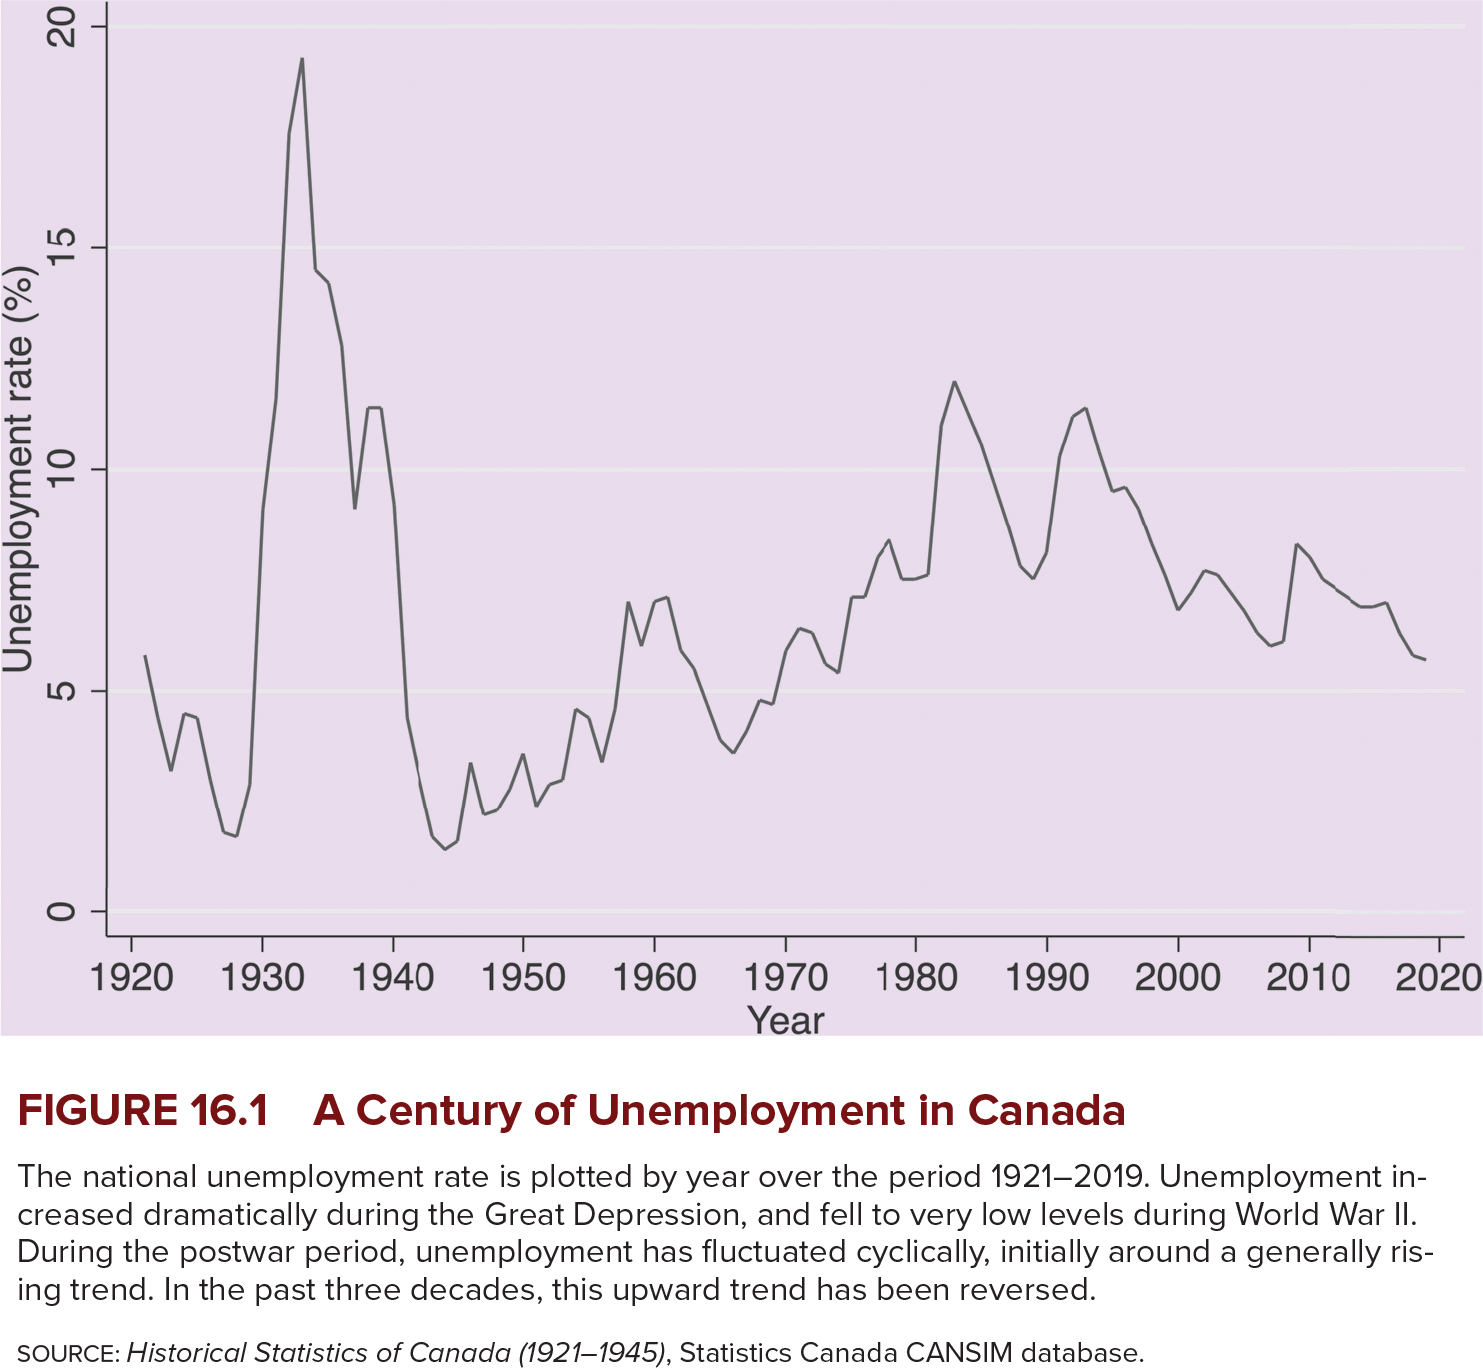
\includegraphics[width=0.68\linewidth]{ben54842_1601}
\end{frame}

% ============================================================
\section{Alternative Indicators}
% ============================================================

\begin{frame}{Alternative Measures of Labour Force Activity}
\transfade
\begin{itemize}[<+->]
  \item \textbf{Unemployment rate:} Fraction of the \emph{labour force} out of work and searching.
  \item \textbf{Employment rate:} Fraction of the \emph{working-age population} employed.
  \item \textbf{Labour force participation rate (LFPR):} Fraction of the \emph{working-age population} in the labour force.
\end{itemize}
\end{frame}

\begin{frame}{Table 16.1: Labour Force Participation, Employment, and Unemployment, Canada, 1946--2019\textsuperscript{a}}
\transfade
\scriptsize
\begin{tabular}{lcccc}
\toprule
\textbf{Year} & \textbf{Labour Force Participation Rate} & \textbf{Employment Rate} & \textbf{Unemployment Rate} & \textbf{Rate of Growth of Employment\textsuperscript{b}} \\
\midrule
1946 & 55.0 & 53.1 & 3.4 &  \\
1956 & 53.5 & 51.7 & 3.4 & 1.8 \\
1966 & 55.1 & 53.1 & 3.6 & 2.5 \\
1973 & 59.7 & 56.4 & 5.6 & 3.0 \\
1981 & 65.0 & 60.0 & 7.6 & 3.2 \\
1989 & 67.2 & 62.1 & 7.5 & 1.8 \\
2000 & 65.9 & 61.4 & 6.8 & 1.2 \\
2008 & 67.6 & 63.4 & 6.1 & 1.8 \\
2019 & 65.7 & 62.0 & 5.7 & 1.0 \\
\bottomrule
\end{tabular}

\vspace{0.25em}
\scriptsize \textit{a.} Canada.\quad \textit{b.} Annual rate of growth of employment.
\end{frame}

% ============================================================
\section{International Comparisons}
% ============================================================

\begin{frame}{International Differences in Unemployment}
\transfade
\begin{itemize}[<+->]
  \item 1950s: U.S. higher than Australia and Japan.
  \item 1973 OPEC shock: rises in several European countries.
  \item 1990s: further increases in France, Germany, Italy.
  \item Since 2000: generally low in English-speaking countries.
  \item 2008--09 crisis: sharp increases across advanced economies.
\end{itemize}
\end{frame}

\begin{frame}{Figure 16.2: Unemployment Rates Across Selected Countries — }
\centering
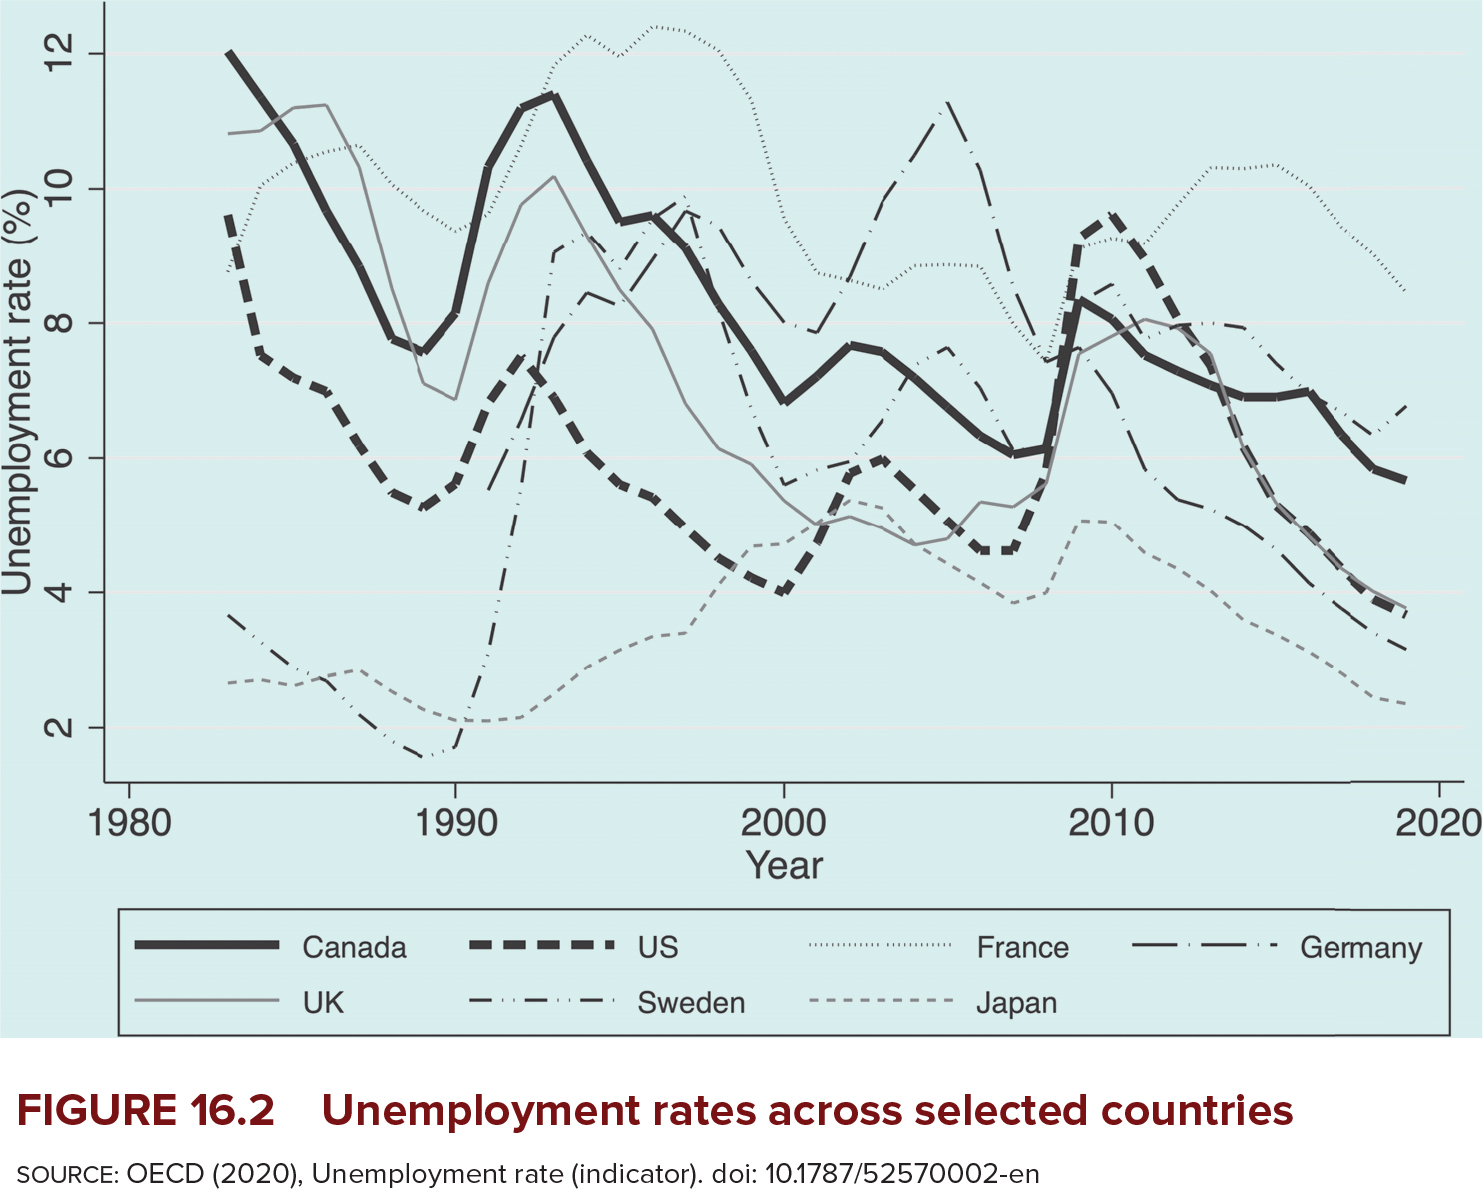
\includegraphics[width=0.68\linewidth]{ben54842_1602}
\end{frame}

% ============================================================
\section{Hidden Unemployment \& Discouraged Workers}
% ============================================================

\begin{frame}{Hidden Unemployment}
\transfade
\begin{itemize}[<+->]
  \item Some without work \emph{want} jobs but are not counted as unemployed.
  \item \textbf{Discouraged workers:} Stop searching when jobs seem unavailable; rise in recessions.
\end{itemize}
\end{frame}

% ============================================================
\section{Labour Force Dynamics}
% ============================================================

\begin{frame}{Labour Market Stocks and Flows}
\transfade
\begin{itemize}[<+->]
  \item Monthly flows among \textbf{employed}, \textbf{unemployed}, and \textbf{not in labour force}.
  \item On average each month: $\sim$235{,}000 unemployed find jobs; $\sim$190{,}000 lose/leave jobs and start searching.
  \item Average net monthly flow $\approx$ 45{,}000; $P(\text{U}\to\text{E})\approx 0.22$.
\end{itemize}
\end{frame}

\begin{frame}{Figure 16.3: Labour Market Stocks and Flows, 1976--1991 }
\centering
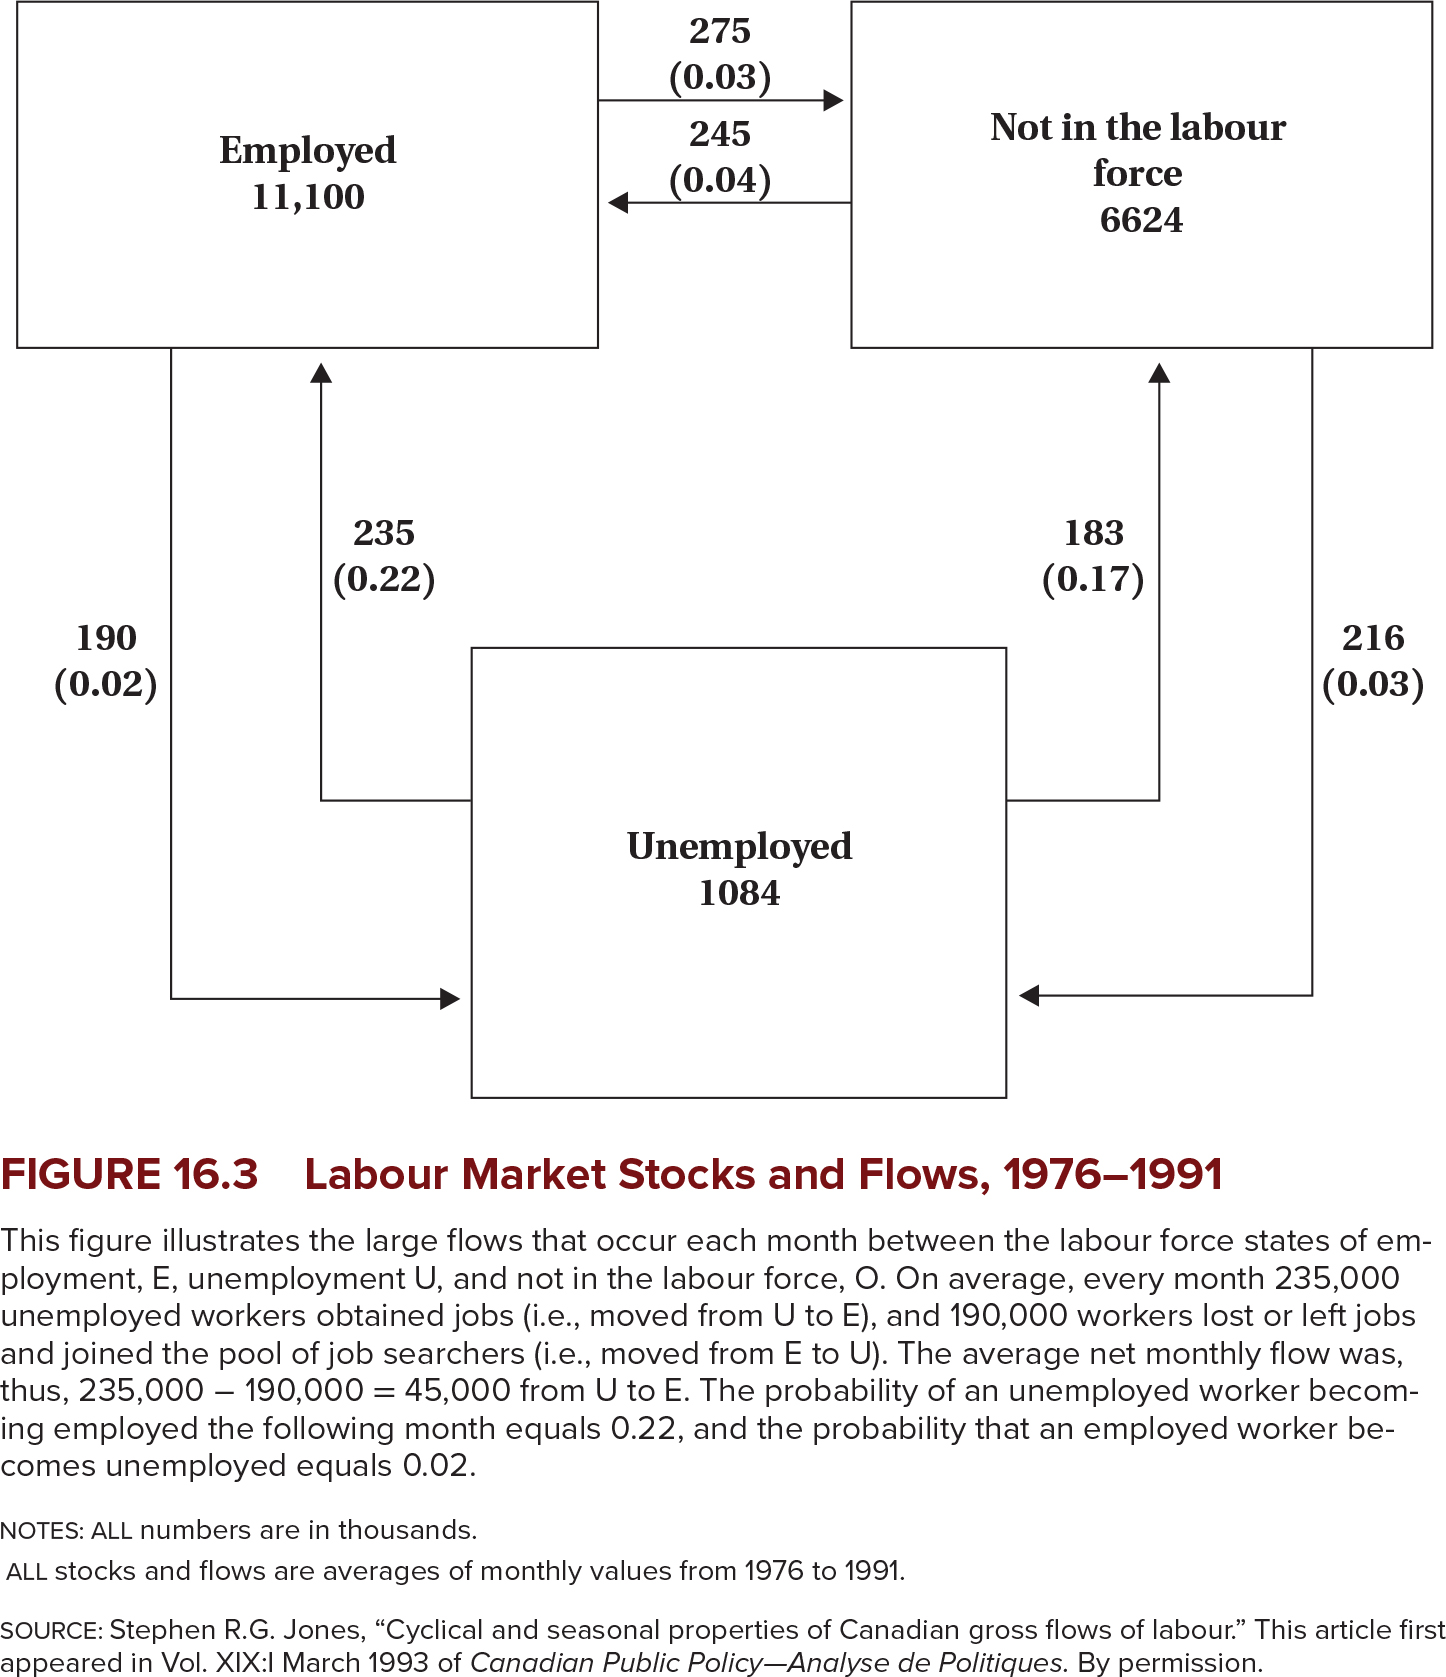
\includegraphics[width=0.63\linewidth]{ben54842_1603}
\end{frame}

\begin{frame}{Table 16.2: Decomposition of Unemployment by Reason, 2005--2019}
\transfade
\scriptsize
\begin{tabular}{lccccc}
\toprule
\multirow{2}{*}{\textbf{Year}} & \textbf{National Unemp.} & \multicolumn{4}{c}{\textbf{Reason for Separation}} \\
\cmidrule(lr){3-6}
 & \textbf{Rate (\%)} & \textbf{Job Losers (\%) Permanent} & \textbf{Temporary Layoffs} & \textbf{Job Leavers (\%)} & \textbf{New Entrants \& Re-entrants (\%)} \\
\midrule
2005 & 6.8 & 28 & 7 & 10 & 42 \\
2006 & 6.3 & 26 & 8 & 11 & 42 \\
2007 & 6.0 & 27 & 7 & 11 & 43 \\
2008 & 6.1 & 29 & 7 & 11 & 44 \\
2009 & 8.3 & 33 & 8 & 8 & 40 \\
2010 & 8.1 & 30 & 6 & 6 & 42 \\
2011 & 7.5 & 27 & 5 & 9 & 43 \\
2012 & 7.3 & 26 & 5 & 8 & 45 \\
2013 & 7.1 & 28 & 5 & 8 & 44 \\
2014 & 6.9 & 28 & 5 & 9 & 44 \\
2015 & 6.9 & 29 & 5 & 8 & 44 \\
2016 & 7.0 & 30 & 4 & 8 & 44 \\
2017 & 6.3 & 27 & 4 & 8 & 47 \\
2018 & 5.8 & 25 & 4 & 9 & 48 \\
2019 & 5.7 & 26 & 4 & 9 & 49 \\
\bottomrule
\end{tabular}
\end{frame}

% ============================================================
\section{Incidence \& Duration}
% ============================================================

\begin{frame}{Incidence and Duration of Unemployment}
\transfade
\begin{itemize}[<+->]
  \item \textbf{Incidence:} Proportion of individuals who \emph{become} unemployed in a period.
  \item \textbf{Duration:} Length of time an individual remains unemployed before exit (to employment or out of labour force).
  \item Both drive the unemployment rate:
\end{itemize}
\[
\textbf{UR} \;=\; \textbf{Incidence} \times \textbf{Duration}\,.
\]
\end{frame}

\begin{frame}{Worked Example: Incidence vs.\ Duration}
\transfade
\small
Two regions have the same unemployment rate, 6\%.\\
Region A: incidence $3\%$ and duration $= 2$ months.\\
Region B: incidence $1.5\%$ and duration $= 4$ months.\\[0.4em]
\textbf{Takeaway:} Same UR can reflect frequent short spells (A) vs.\ fewer but longer spells (B) $\Rightarrow$ policy focus differs (job-finding vs.\ income support).
\end{frame}

\begin{frame}{Table 16.3: Incidence and Duration of Unemployment by Age and Sex, Canada, 2019}
\transfade
\scriptsize
\begin{tabular}{llcccc}
\toprule
\textbf{Sex} & \textbf{Age Group} & \textbf{Unemployment Rate} & \textbf{Incidence Rate} & \textbf{Duration (Months)} & \textbf{Unemployed $>$ 6 Months (\%)} \\
\midrule
Men & 15--24 & 12.3 & 6.1 & 2.0 & 7.5 \\
 & 25--44 & 5.3 & 1.9 & 2.8 & 14.8 \\
 & 45 + & 4.8 & 1.4 & 3.4 & 23.6 \\
 & All & 6.0 & 2.3 & 2.7 & 15.8 \\
\midrule
Women & 15--24 & 9.7 & 5.1 & 1.9 & 5.9 \\
 & 25--44 & 5.3 & 1.9 & 2.8 & 13.2 \\
 & 45 + & 4.2 & 1.3 & 3.3 & 22.1 \\
 & All & 5.3 & 2.1 & 2.5 & 14.2 \\
\bottomrule
\end{tabular}
\end{frame}

\begin{frame}{Changing Perspectives on Unemployment}
\transfade
\begin{itemize}[<+->]
  \item The labour force is \textbf{highly dynamic}.
  \item Roughly half of inflows to unemployment are job losers.
  \item Even in 2010 (above-normal unemployment), average duration $\approx$ 3 months; about one-fifth of spells $>$ 6 months.
  \item Highest unemployment rates are in younger groups, who also have \textbf{shorter} durations but \textbf{higher} incidence.
\end{itemize}
\end{frame}

\begin{frame}{Table 16.4: International Differences in Long-Term Unemployment}
\transfade
\scriptsize
\begin{tabular}{lcc}
\toprule
\textbf{Long-Term Unemployment as a \% of Total Unemployment} & \textbf{1999 (12+ months)} & \textbf{2019 (12+ months)} \\
\midrule
Canada & 11.7 & 8.5 \\
France & 40.4 & 38.8 \\
Germany & 51.8 & 38.1 \\
Japan & 22.4 & 32.3 \\
Sweden & 30.1 & 12.1 \\
United Kingdom & 29.6 & 25.1 \\
United States & 6.8 & 12.7 \\
\bottomrule
\end{tabular}
\end{frame}

% ============================================================
\section{Interpreting the Unemployment Rate}
% ============================================================

\begin{frame}{Unemployment Rate as a Summary Statistic}
\transfade
\begin{itemize}[<+->]
  \item Widely used indicator of the \textbf{aggregate state} of the economy.
  \item Signals tightness/looseness of the labour market; rises in low/negative growth.
  \item Measures unused labour supply, but may not capture all \textbf{hardship} (e.g., hidden unemployment).
\end{itemize}
\end{frame}

% ============================================================
\section{Chapter Summary}
% ============================================================

\begin{frame}{Summary}
\transfade
\begin{itemize}[<+->]
  \item Unemployment definitions and measurement via the LFS.
  \item Canada’s historical experience and cross-country differences.
  \item Hidden unemployment and discouraged workers matter for interpretation.
  \item Stocks, flows, and $\text{UR} = \text{Incidence} \times \text{Duration}$ clarify dynamics.
  \item International evidence on long-term unemployment highlights structural differences.
\end{itemize}
\end{frame}

\begin{frame}
\centering
\Huge{\textbf{Thank You!}} \\

\end{frame}

\end{document}
